\section{Working with Controls}
\label{tutorial_04}

A Control is a graphical representation of some aspects of the model. Typically it uses images, labels, shapes or buttons to represent information. For instance, if we model a traffic light with the two colors green and red, we might simply use a circle shape for each color.

Since we want to visualize a waterboiler we have to add some nice images which represent the different states of the model like the open/closed cap. Note that this step is optional since we could use the other predefined Controls like shapes to represent the model. However, we want to cover all features in this tutorial. For this reason we created the images in order to represent the different states of the cap or the waterboiler respectively as shown in table \ref{table_tut_04_waterboilerimages}.

\begin{table}[h!]
\begin{center}
    \begin{tabular}{ | c | c |}
    \hline
	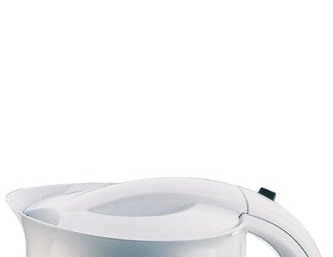
\includegraphics{img/tutorial/tut_04_capclosed.jpg} & 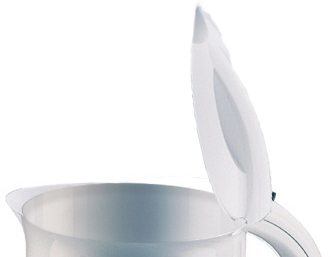
\includegraphics{img/tutorial/tut_04_capopen.jpg} \\ \hline
	Image representing the closed cap & Image representing the open cap  \\ \hline
	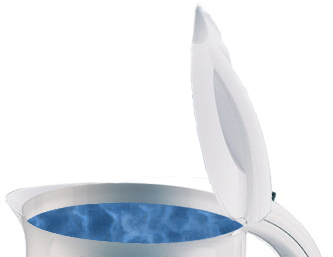
\includegraphics{img/tutorial/tut_04_capfull.jpg} & 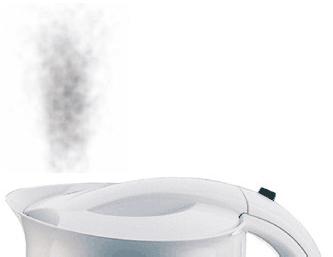
\includegraphics{img/tutorial/tut_04_capon.jpg} \\ \hline
	Image representing the full cap & Image representing the waterboiler after switching it on   \\ \hline
    \end{tabular}
\caption{Images representing the different states of the Waterboiler model}
\label{table_tut_04_waterboilerimages}
\end{center}
\end{table}

In order to use the images in our visualization we have to add them to our project. This is done with the help of the Library View (\ref{library_view}) which allows us to administrate resources like images with useful features like preview and import/delete functions. 

\subsection{Systems Development}

Text ...
